\documentclass{beamer}
\usetheme{Warsaw}

\usepackage[utf8]{inputenc}
\usepackage{fancybox}
\usepackage{multimedia} 
\usepackage{subfig}
\usepackage{amsmath}

\usepackage[all]{xy}
\begin{document}


\title[Computergrafik] % (optional, only for long titles)
{Computergrafik

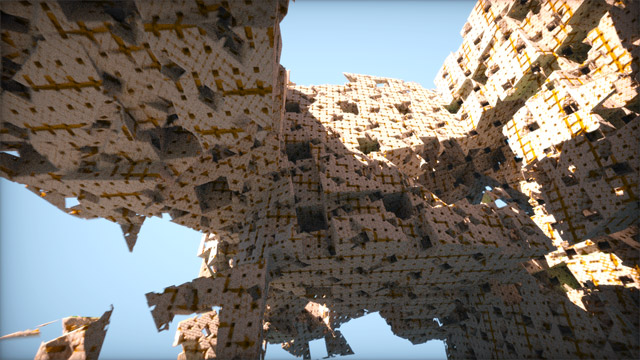
\includegraphics[scale=0.36]{images/cover}
}
\subtitle{}
\author[Dr. Johannes Riesterer] % (optional, for multiple authors)
{Dr.  rer. nat. Johannes Riesterer}

\date[KPT 2004] % (optional)
{}

\subject{Computergrafik}

\begin{frame}
    \frametitle{Lichtmodelle}
\framesubtitle{}
    \begin{block}{Licht}
\begin{center}
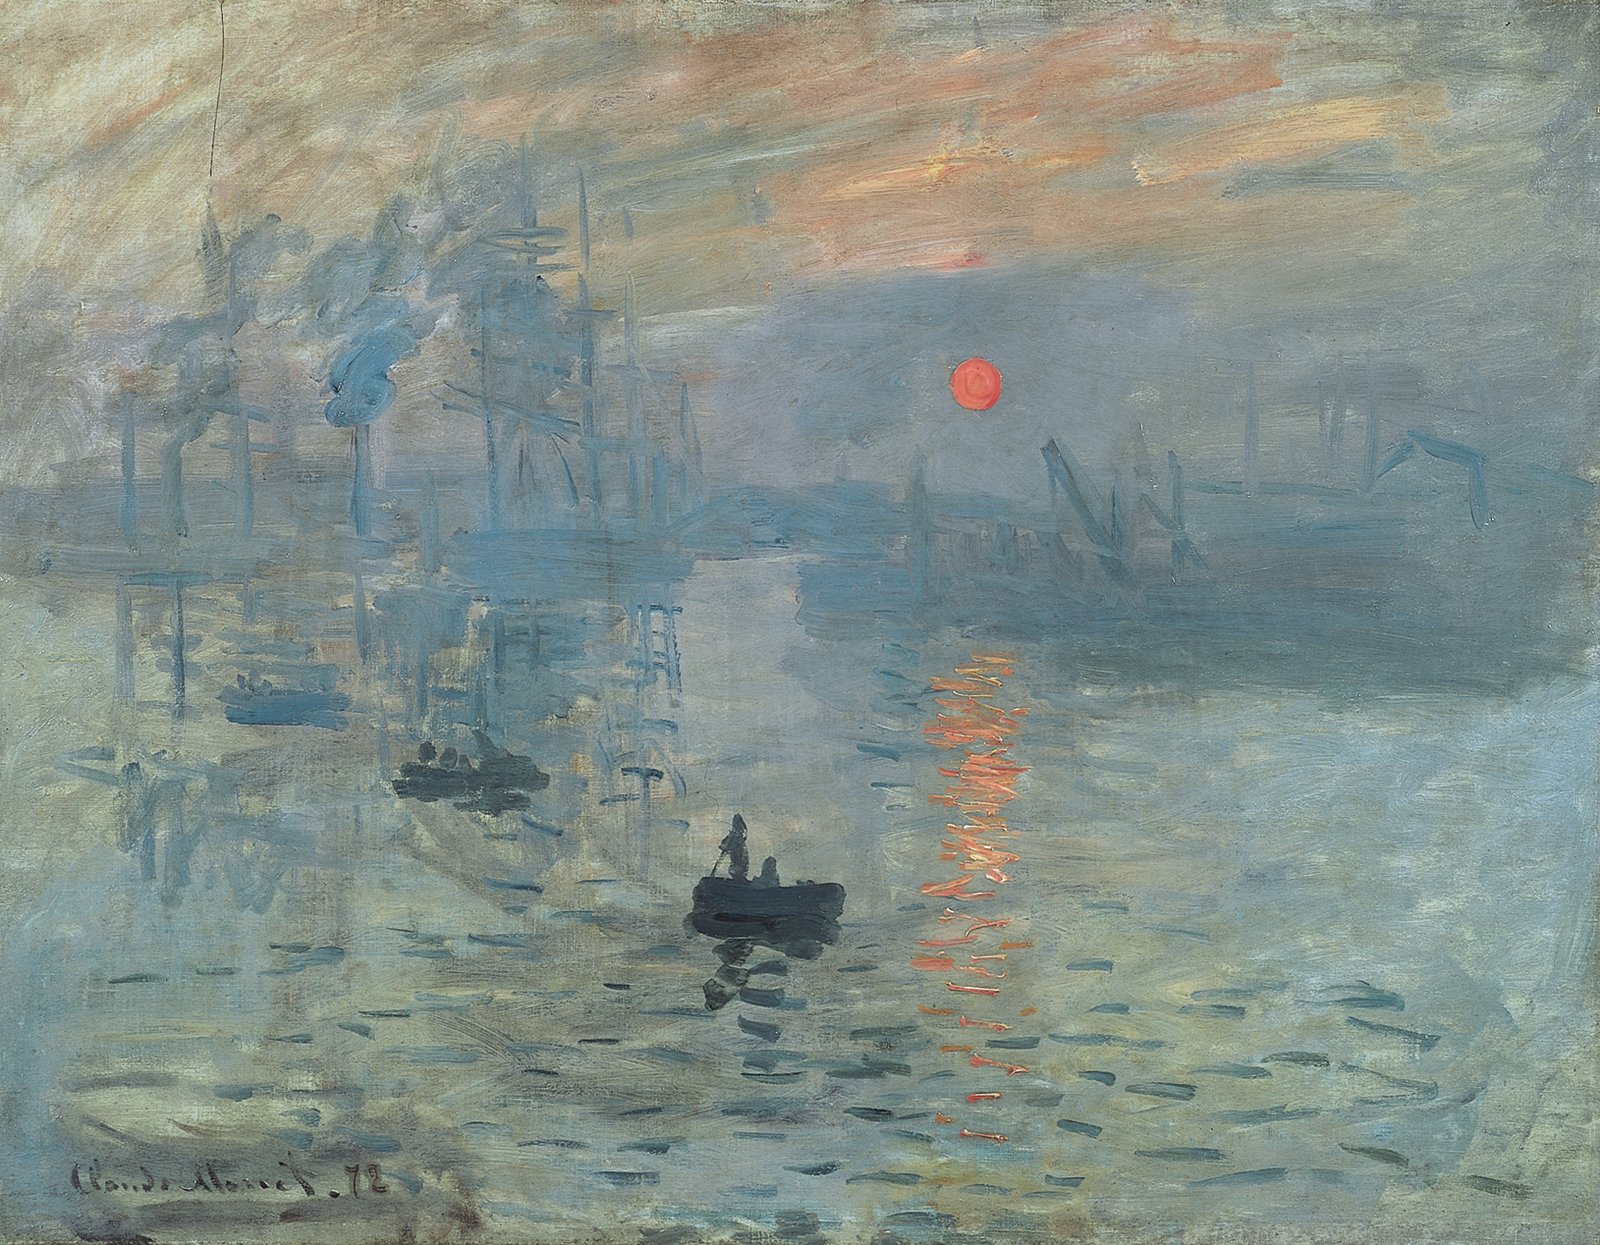
\includegraphics[scale=0.65]{images/monet}
\end{center}
\end{block}

\end{frame}

\begin{frame}
    \frametitle{Lichtmodelle}
\framesubtitle{}
\begin{center}
    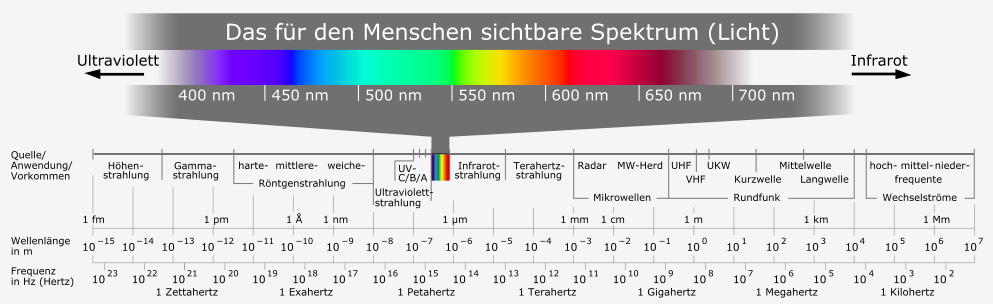
\includegraphics[width=1.0\textwidth]{images/Electromagnetic_spectrum_c.png}
\end{center}
\begin{block}{Licht}
Licht ist sowohl eine elektromagnetische Welle, als auch ein Teilchen, genannt Photon. Es breitet sich mit Lichtgeschwindigkeit $c=299 792 458 m/s$ aus. 
Die Energie eines Photons ist 
durch $E=h \cdot f$, wobei  $h$ das konstante Planksche Wirkungsquantum und $f$ die Frequenz der Welle ist.
\end{block}
\end{frame}

\begin{frame}
    \frametitle{Lichtmodelle}
\framesubtitle{}
\begin{center}
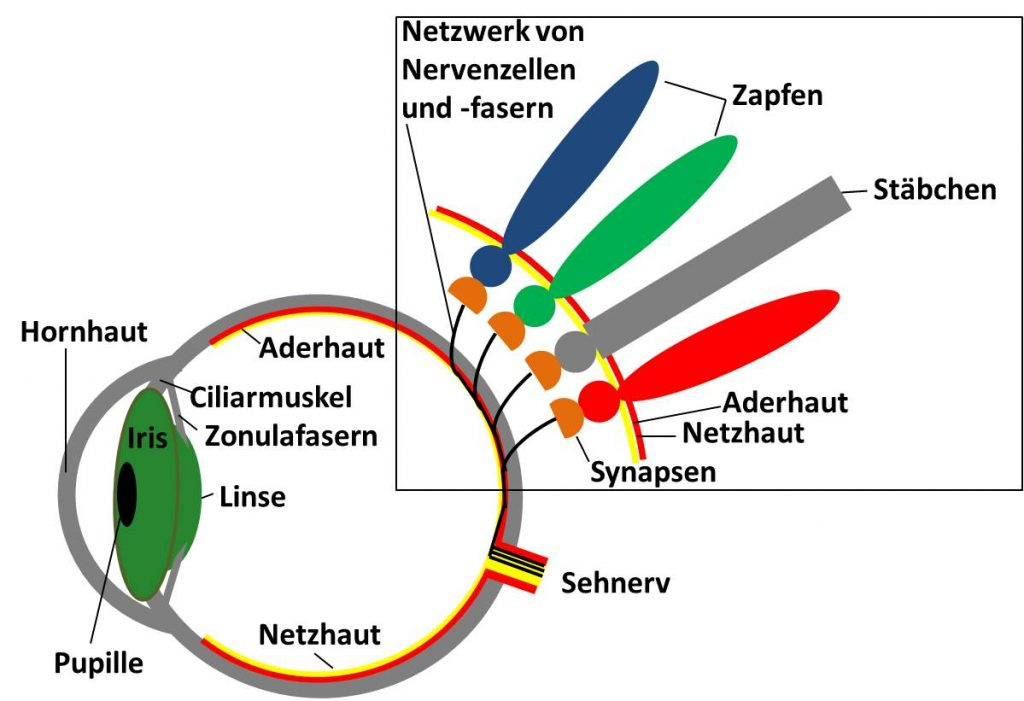
\includegraphics[scale=0.35]{images/Auge}
\end{center}

\end{frame}

\begin{frame}
    \frametitle{Lichtmodelle}
\framesubtitle{}
\begin{center}
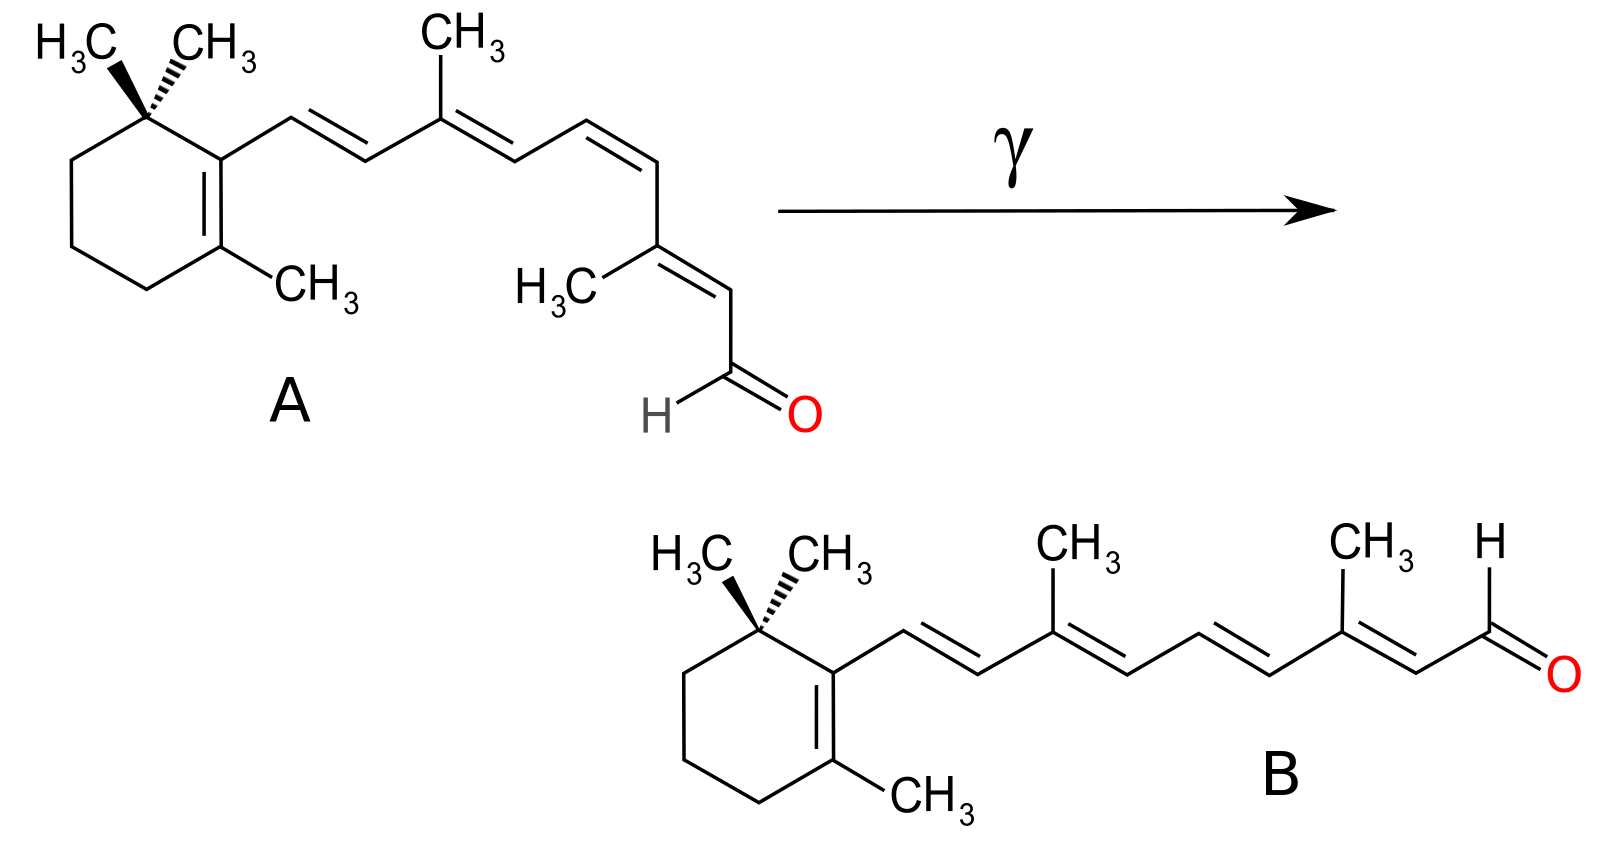
\includegraphics[scale=0.09]{images/RetinalCisandTrans} 
\end{center}
    \begin{block}{Farbwahrnehmung}
Trifft ein Photon mit passender Energie auf das Retinal-Molekül, so ändert es seine räumliche Struktur. Diese Strukturveränderung wird als primäre photochemische Reaktion bezeichnet. Sie dauert etwa $2 \cdot 10^{-14}s$  und löst mehrere nachgeordnete Prozesse in der Sinneszelle aus, die das Signal erheblich verstärken und schließlich in einer Veränderung ihres Membranpotentials münden, welches dann eine nervliche Signalkette auslöst. 
\end{block}
\end{frame}


\begin{frame}
    \frametitle{Lichtmodelle}
\framesubtitle{}
\begin{center}
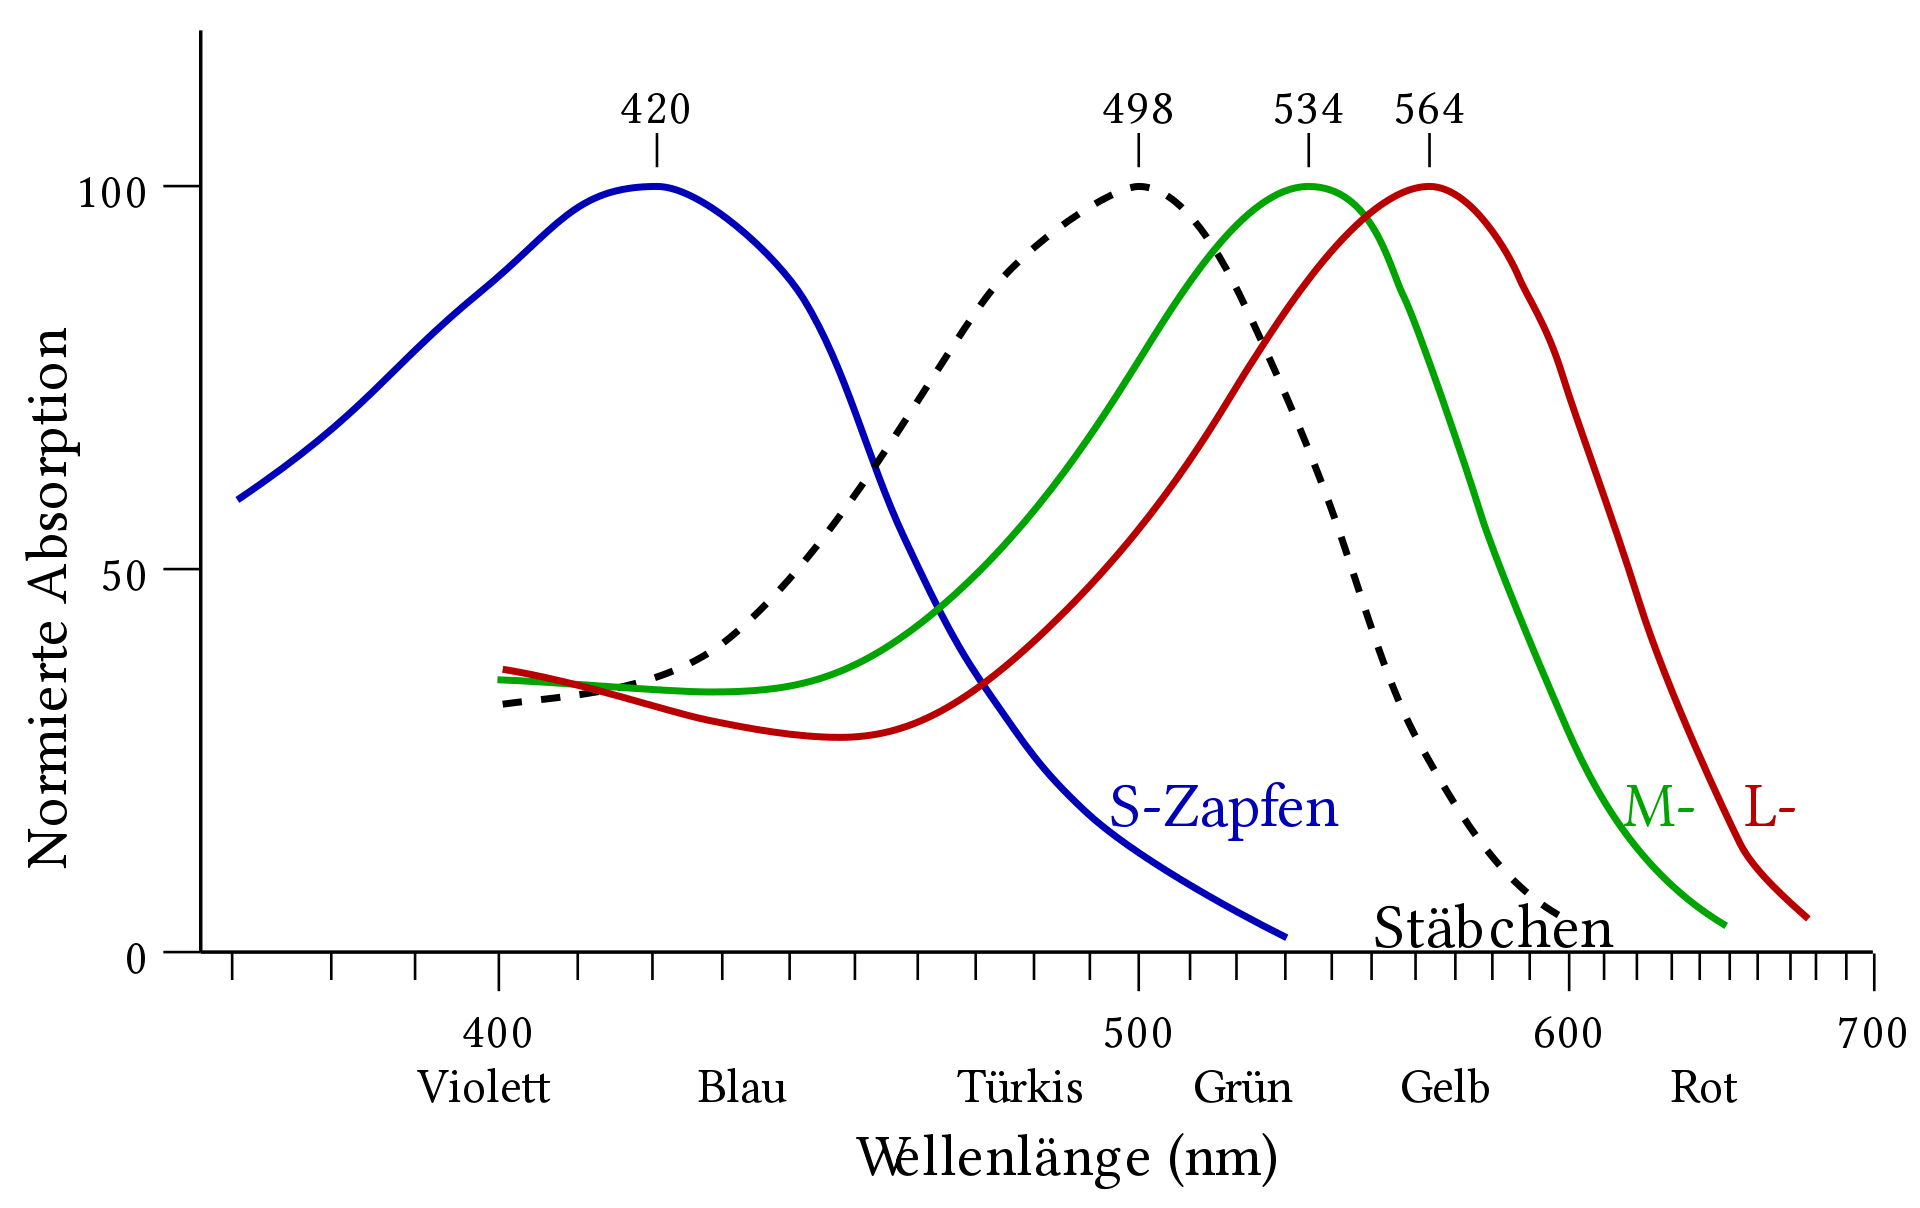
\includegraphics[scale=0.14]{images/farbwahrnehmung}
\end{center}
    \begin{block}{Farbwahrnehmung}
Das sichtbare Licht liegt zwischen 380 nm und 780 nm.

\end{block}
\end{frame}




\begin{frame}
    \frametitle{Lichtmodelle}
\framesubtitle{}
\begin{center}
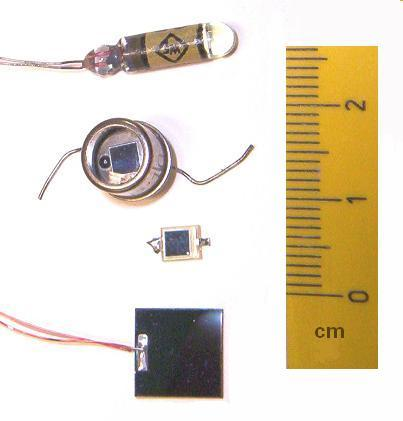
\includegraphics[scale=0.9]{images/Fotodiode}
\end{center}
    \begin{block}{Photodioden}
Photodioden werden aus Elementhalbleitern hergestellt.
Treffen Photonen ausreichender Energie auf das Material der Diode, so werden Ladungsträger (Elektron-Loch-Paare) erzeugt. 
In der Raumladungszone driften die Ladungsträger schnell entgegen der Diffusionsspannung in die gleichartig dotierten Zonen und führen zu einem Strom. 
\end{block}
\end{frame}






\begin{frame}
    \frametitle{Lichtmodelle}
\framesubtitle{}
\begin{center}
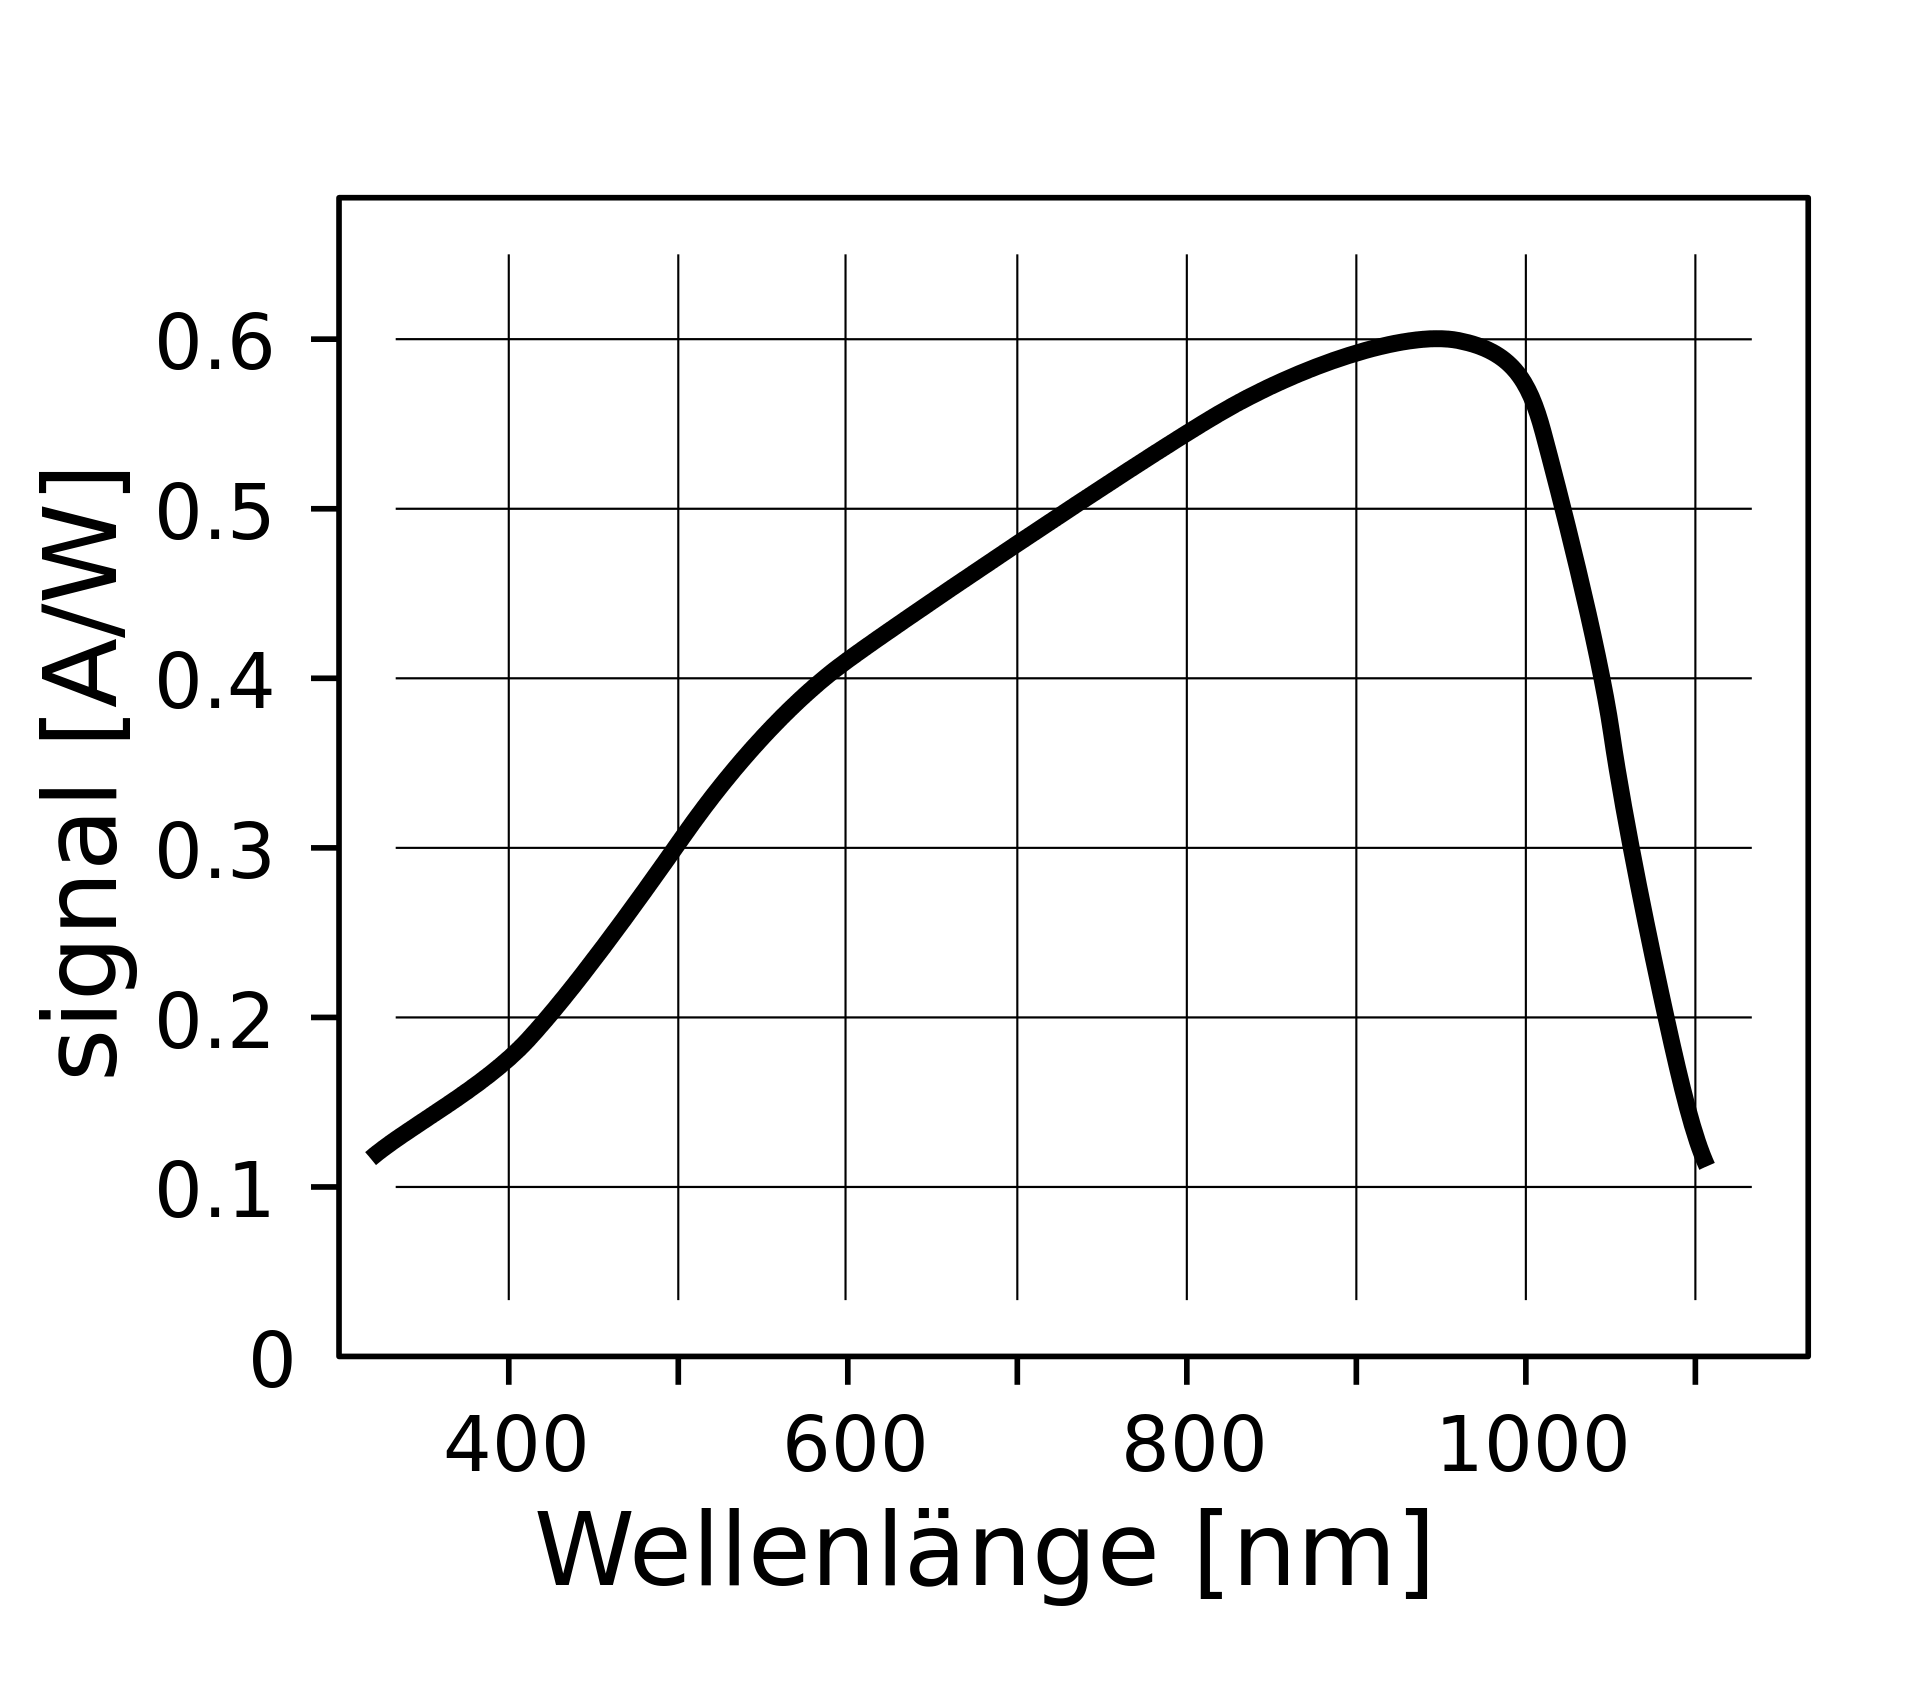
\includegraphics[scale=0.1]{images/photodiode_strom}
\end{center}

\end{frame}




\begin{frame}
    \frametitle{Photometrie}
\framesubtitle{}
  \begin{center}

    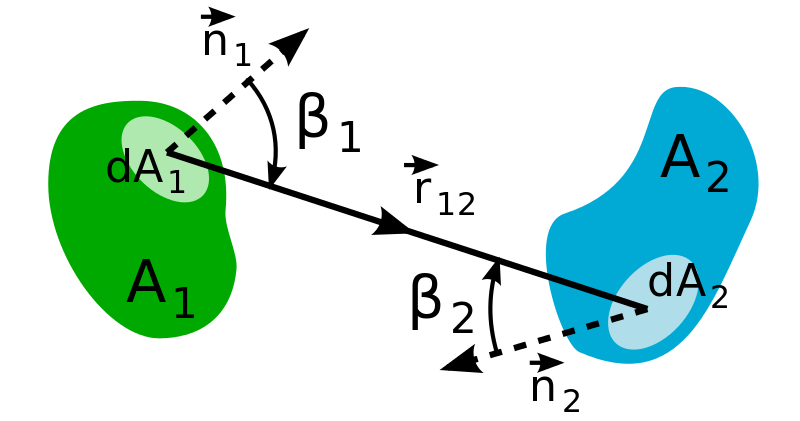
\includegraphics[width=0.45\textwidth]{images/Fotometrisches_Grundgesetz_Schema.png}
\end{center}

\end{frame}


\begin{frame}
    \frametitle{Photometrie}
\framesubtitle{}
\begin{center}
    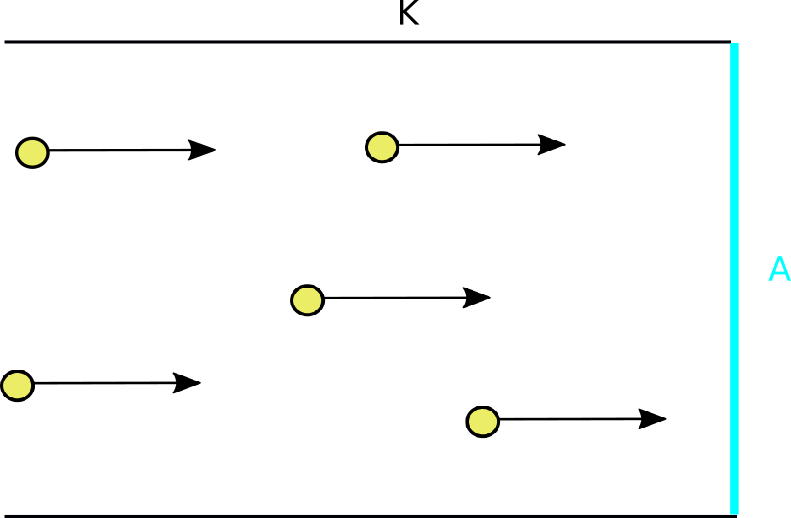
\includegraphics[width=0.4\textwidth]{images/Partikelstrom.png}
\end{center}
\begin{block}{ Strahldichte}

Durch einen Kanal $K$ bewegen  sich Teilchen mit gleichförmiger Geschwindigkeit $L$ (Lichtgeschwindigkeit)  und  Dichte $\eta$.
Die Anzahl der Teilchen $N$, die die Fläche $A$ bezüglich eines Zeitintervalles $[0,t]$ passieren, ist gegeben durch
\begin{align}
& N_A([0,t]) := \eta * ||L||  *   \text{Flächeninhalt}(A) *   t 
\end{align}
\end{block}
\end{frame}

\begin{frame}
    \frametitle{Photometrie}
\framesubtitle{}

\begin{center}

    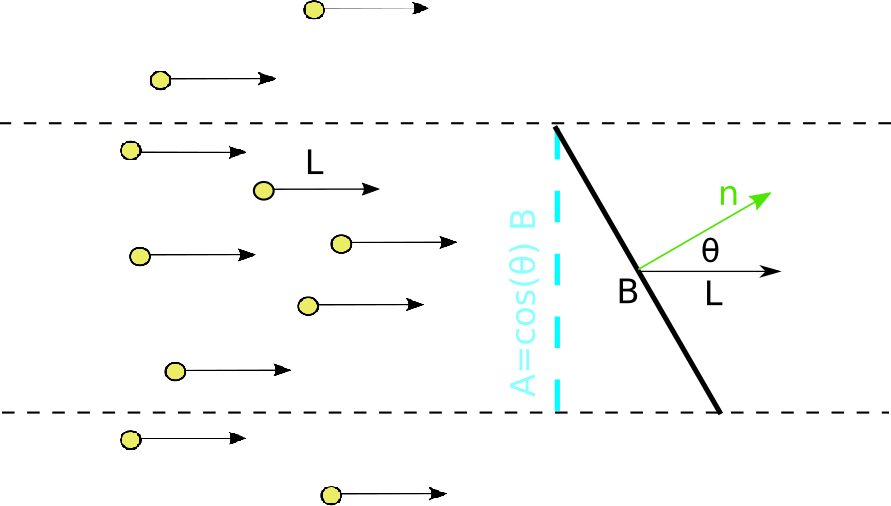
\includegraphics[width=0.5\textwidth]{images/Strahldichte.png}
\end{center}


\begin{block}{Strahldichte}
 Betrachtet man die allgemeinere Situation eines Flächenstückes $B$, so ist die Anzahl gegeben durch 
\begin{align}
N_B([0,t]) := \eta * ||L||  * \cos(\theta) *  \text{Flächeninhalt} (B) * t
 \end{align}


\end{block}
\end{frame}




\begin{frame}
    \frametitle{Photometrie}
\framesubtitle{}

\begin{block}{Strahldichte}
Bezeichnen wir mit 
\begin{align*}
L(B) = \frac{d}{dt \cdot \cos(\theta)}N_B([0,t]) = \eta * ||L||  *  \text{Flächeninhalt} (B) \; , 
 \end{align*}

so erhalten wir die   Strahldichte als Grenzwert
\begin{align*}
L(x, n):= \lim_{B -> x} L(B)
 \end{align*}
bei dem die Fläche $B$  zu einem Punkt $x$ zusammengezogen wird.  Die Strahlungsleistung aus einer Richtung $n$  am Punkt $x$ berechnet sich demnach durch $I(x, n) = L(x, n) \cdot \cos(\theta)$, was auch als Lambertsches Cosinusgesetz bezeichnet wird.
\end{block}
\end{frame}
 

\begin{frame}
    \frametitle{Photometrie}
\framesubtitle{}
\begin{block}{Strahlungsleistung}

Die Strahlungsleistung $\phi = \frac{d Q}{dt}$ ist die von einem Photonenstrom übertragenen Energie $Q$ pro Zeit. 
Für monochromes Licht mit der Frequenz $f$ und Teilchenstrom $ \frac{d N}{dt} $ ergibt sich mit obigen Überlegungen $\phi = h \cdot  \frac{d N}{dt}  \cdot f$.
\end{block}
\end{frame}




\begin{frame}
    \frametitle{Photometrie}
\framesubtitle{}
\begin{block}{Fläche}

Ein Fläche (Parametrisierung) ist  eine  Abbildung
\begin{align*}
s: U \subset \mathbb{R}^2 \to \mathbb{R}^3 \\
s(u,v) := \begin{pmatrix} x(u,v) \\ y(u,v) \\ z(u,v) \end{pmatrix} 
\end{align*} 
bei der die Abbildungen $x, y, z : U \subset \mathbb{R}^2 \to \mathbb{R}$ stetig sind. Sie heißt differenzierbar, falls die partiellen Ableitungen
\begin{align*}
\frac{\partial}{\partial u} s(u,v) = \begin{pmatrix}  \frac{\partial}{\partial u} x(u,v) \\  \frac{\partial}{\partial u} y(u,v) \\  \frac{\partial}{\partial u} z(u,v) \end{pmatrix}, \;
\frac{\partial}{\partial v} s(u,v) =  \begin{pmatrix} \frac{\partial}{\partial v} x(u,v) \\ \frac{\partial}{\partial v} y(u,v) \\ \frac{\partial}{\partial v} z(u,v) \end{pmatrix}
\end{align*}
existieren. 
\end{block}
\end{frame}


\begin{frame}
    \frametitle{Photometrie}
\framesubtitle{}
\begin{block}{Tangentialraum}

Die Ebene 
\begin{align*}
T_s(u,v) :=  \{ s(u,v) + \lambda \cdot \frac{\partial}{\partial u} s(u,v) + \mu \cdot \frac{\partial}{\partial v} \; | \; \lambda, \mu \in \mathbb{R} \}
\end{align*}
heißt Tangentialebene am Punkt $(u,v)$ und  der Vektor 
\begin{align*}
n (u,v):= \frac{\partial}{\partial u} s(u,v) \times \frac{\partial}{\partial v} s(u,v) \; ,
\end{align*}
welcher Senkrecht auf dieser Ebene steht,  die Normale.
\end{block}
\end{frame}

\begin{frame}
    \frametitle{Photometrie}
\framesubtitle{}
\begin{block}{Oberflächenintegral}

Das OberflächenIntegral ist definiert durch
\begin{align*}
\int_S d \omega:= \int_U ||n(u,v)|| \; dU \;.
\end{align*} 
und  analog
\begin{align*}
\int_S f \;  d \omega:= \int_U f(s(u,v)) \cdot ||n(u,v)|| \; dU \;.
\end{align*} 
für eine Funktion $f: S \to \mathbb{R}$.
Man nennt $d \omega$ beziehungsweise $ ||n(u,v)||$ das infinitessimale Flächenelement.
\end{block}
\end{frame}

\begin{frame}
    \frametitle{Photometrie}
\framesubtitle{}
\begin{block}{Fubini}
Ist $U = U_1 \times U_2 \in \mathbb{R}^2$ und $f: U \to \mathbb{R}$ eine integrierbare Funktion, so gilt
\begin{align*}
\int_U f \; d(U_1 \times U_2) = \int_{U_1} \int_{U_2} f  \;  dU_2 dU_1   = \int_{U_1} \int_{U_2} f  \;  dU_1 dU_2 \;.
\end{align*} 
\end{block}
\end{frame}


\begin{frame}
    \frametitle{Photometrie}
\framesubtitle{}
\begin{block}{Die  Sphäre $S^2$}
\begin{align*}
& s:  [0, \pi) \times  [0, 2 \pi)  \to \mathbb{R}^3 , \;
  s(u,v) :=  
 \begin{pmatrix}  \sin(u) \cos(v) \\   \sin(u) \sin(v) \\   \cos(u)  \end{pmatrix} \\
& \frac{\partial}{\partial u} s(u,v) =  \begin{pmatrix}  \cos(u) \cos(v) \\   \cos(u) \sin(v) \\   -\sin(u)  \end{pmatrix} , 
\frac{\partial}{\partial v} s(u,v) =  \begin{pmatrix}  -\sin(u) \sin(v) \\   \sin(u) \cos(v) \\   0  \end{pmatrix} \\
& ||\frac{\partial}{\partial u} s(u,v) \times \frac{\partial}{\partial v} s(u,v) || = sin(u)
\end{align*} 
\begin{align*}
& \int_{S^2} d\omega  = \int_{[0, \pi) \times  [0, 2 \pi) } sin(u) d(u \times v) =   \int_{[0, 2 \pi) }   \int_{[0, \pi) } sin(u) du dv \\ 
& = 4 \pi
\end{align*} 

\end{block}
\end{frame}

\begin{frame}
    \frametitle{Photometrie}
\framesubtitle{}
  \begin{center}

    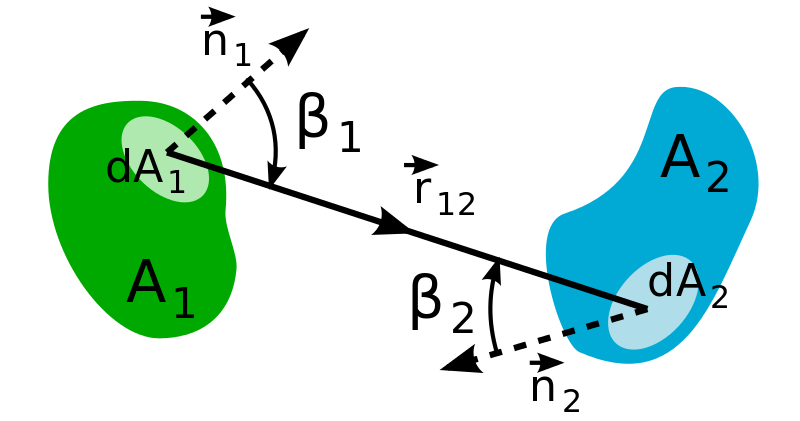
\includegraphics[width=0.45\textwidth]{images/Fotometrisches_Grundgesetz_Schema.png}
\end{center}


\begin{block}{Photometrisches Grundgesetz}

Die Strahlungsleistung $\phi:= \frac{ \partial Q}{\partial t}$, die von einer abstrahlenden Fläche $A_2$  auf eine Fläche $A_1$ übertragen wird, berechnet sich durch
\begin{align}
\phi = \int_{A_1} \int_{\pi_s(A_2)} L(x, \omega)\cdot \cos(\beta_1) d\omega  dA_1   \; ,
\end{align}
wobei $\beta_1$ der Winkel zwischen der Flächennormale am Punkt $x$ und der Richtung $\omega$ ist und $\pi_s(A_2)$ das sphärische Bild von $A_2$ ist.
\end{block}
\end{frame}




\begin{frame}
    \frametitle{Photometrie}
\framesubtitle{}
\begin{center}
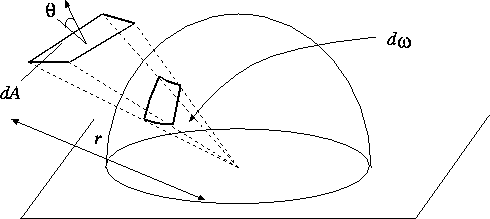
\includegraphics[scale=0.30]{images/solidangle}
\end{center}

\begin{block}{Transformationsformel}


\begin{align}
& d\omega =  \frac{1}{r^2} \cdot  \cos(\theta) dA, \;  \pi(x):=  \frac{x}{||x||}  \\
& V(x,y) := \begin{cases}
1 \text{ falls } \overline{xy} \cap (A -\{x,y\}) = \emptyset \\
0 \text{ sonst }
\end{cases} \\
& \int_{\pi(A)} f \cdot   d\omega  =  \int_{A} f  \cdot \frac{1}{r^2} \cdot  \cos(\theta) \cdot V(a, 0)  \; dA \; ,
\end{align}


\end{block}
\end{frame}




\begin{frame}
    \frametitle{Photometrie}
\framesubtitle{}
\begin{block}{Reflektionsgesetz}

\begin{align*}
\underbrace{L_r(x, \omega_r)}_{\substack{\text{Reflektierte Strahlung} \\ \text{in Richtungen $\omega_r$}}} =\underbrace{\int_{H^2} \underbrace{f_r (x, \omega, \omega_r)}_{\substack{\text{Reflektionseigenschaft} \\ \text{des Materials}}} \cdot  \underbrace{L_i(x, \omega) \cdot  \cos(\theta) }_{\substack{\text{Eingehende Strahlung} \\ \text{aus Richtung $\omega$}}} d\omega}_{\substack{\text{Summation über  alle } \\ \text{eingehenden Richtungen $\omega$}}} 
\end{align*}
  \begin{center}
    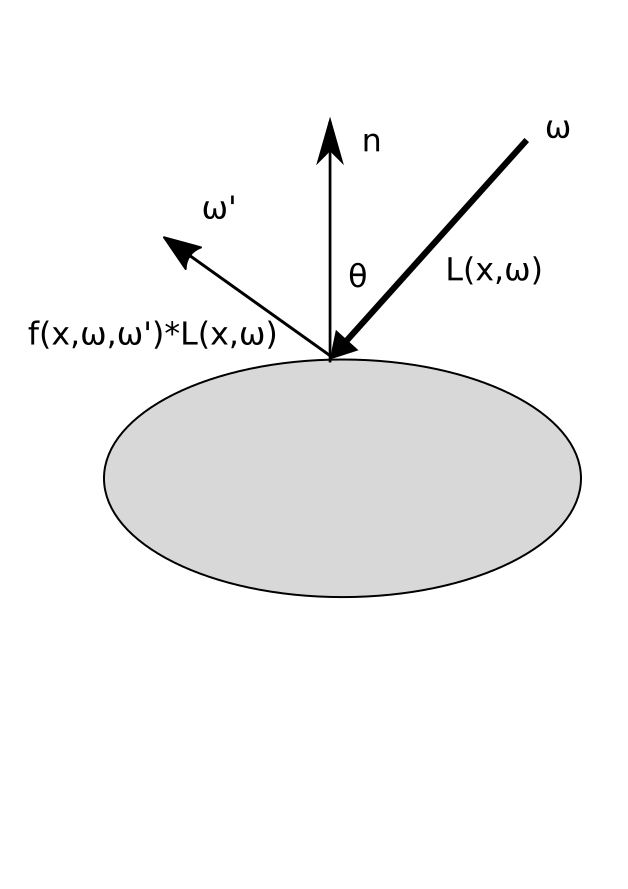
\includegraphics[width=0.3\textwidth]{images/brdf.png}
\end{center}
\end{block}
\end{frame}


\begin{frame}
    \frametitle{Raytracing}
\framesubtitle{}
\begin{block}{Rendergleichung}

\begin{align}
L_o(x, \omega_o) = L_e(x, \omega_o)  + \displaystyle \int_{H^2}f_r (x, \omega, \omega_0) \cdot L_i(x, \omega)  \cdot  \cos(\theta) d\omega \; ,
\end{align}
Ausgehend (\textbf{o}ut) = Emission (\textbf{e}mission) + Reflektion
\end{block}
\end{frame}



\begin{frame}
    \frametitle{Raytracing}
\framesubtitle{}

  \begin{center}
    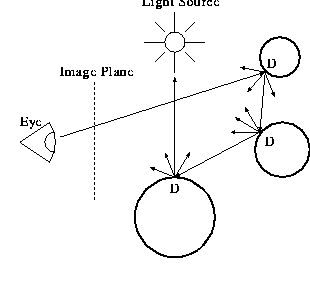
\includegraphics[width=0.7\textwidth]{images/rayTracing}
\end{center}

\end{frame}



\begin{frame}
    \frametitle{Raytracing}
\framesubtitle{}
\begin{block}{Rendergleichung 2-te Form}
 $\Omega$  Menge aller Flächen  in der Szene.
\begin{align*}
& V(x,y) := \begin{cases}
 1 \text{ falls } \overline{xy} \cap (\Omega -\{x,y\}) = \emptyset \\
0 \text{ sonst }
\end{cases} \\
& L_i(x, \omega_y) = V(x,y) \cdot L_o(y, \omega_x) \text{ (Energieerhaltung)} \\
& d\omega =  \frac{1}{||x -y||^2} \cdot  \cos(\theta_y) dA_y \\
& G(x,y) := V(x,y)  \frac{ \cos(\theta_x) \cdot  \cos(\theta_y)}{||x -y||^2} \\
& L_o(x, \omega_o) = L_e(x, \omega_o)  + \displaystyle \int_{\Omega} f_r (x, \overline{xy}, \omega_o) \cdot   L_o(y, \overline{xy})  \cdot  G(x,y) \cdot   dA_y \; .
\end{align*} 
\end{block}
\end{frame}


\begin{frame}
    \frametitle{Raytracing}
\framesubtitle{}
\begin{block}{Pfadformulierung}
\begin{align*}
&(T \circ  L)(x, \omega) :=  \displaystyle \int_{H^2}f_r (x, \omega, \omega_0) \cdot L(x, \omega)  \cdot  \cos(\theta) d\omega \; , \\
&L_e = (id - T) \circ L \; . \\
&L = (id - T)^{-1} \circ L_e  \\
&(id - T)^{-1}= \sum_{i= 0}^{\infty} T^i  \; .
\end{align*}

\end{block}
\end{frame}

\begin{frame}
    \frametitle{Monte Carlo Integration}
\framesubtitle{}
\begin{block}{Wahrscheinlichkeitsraum}
\begin{itemize}
\item  Menge $\Omega \subset \mathbb{R}^n$ deren Teilmengen Ereignisse genannt werden.
\item Funktion $\rho : \Omega \to \mathbb{R}$ mit $\int_{\Omega} \rho(\omega) d\omega = 1$ welche auch Wahrscheinlichkeitsdichte genannt wird.
\item Eine Abbildung $X: \Omega \to \mathbb{R}$ wird Zufallsvariable genannt.
\end{itemize}

Ist $X: \Omega \to \mathbb{R}$ eine  Zufallsvariable, dann heißt
\begin{align}
\mathbb{E}[X] := \int_{\Omega} X(\omega) \cdot \rho(\omega) d\omega 
\end{align}
Erwartungswert.
\end{block}
\end{frame}

\begin{frame}
    \frametitle{Monte Carlo Integration}
\framesubtitle{}
\begin{block}{Gesetz der großen Zahlen}
Ist $X: \Omega \to \mathbb{R}$ eine  Zufallsvariable mit Wahrscheinlichkeitsdichte $\rho: \Omega \to [0,1]$ und $\{ \omega_1, \cdots, \omega_N \}$ eine Stichprobe für $\rho$, so gilt:
\begin{align}
\frac{1}{N} \sum_{i= 0}^{N} X(\omega_i) \xrightarrow{ N \to \infty } \mathbb{E}[X] \text{ (in Wahrscheinlichkeit)}
\end{align}
\end{block}
\end{frame}

\begin{frame}
    \frametitle{Monte Carlo Integration}
\framesubtitle{}
\begin{block}{Stochastische Integration}

Ist $f: S \subset \Omega \to \mathbb{R}$ eine Funktion, so gilt für eine beliebige Wahrscheinlichkeitsdichte  $\rho: \Omega \to [0,1]$ und eine Stichprobe 
 $\{ \omega_1, \cdots, \omega_N \}$
\begin{align}
\frac{1}{N} \sum_{i= 0}^{N}  \frac{f(\omega_i)}{\rho(\omega_i)} \xrightarrow{ N \to \infty } \int_{\Omega} f(\omega) d\omega \text{ (in Wahrscheinlichkeit)} \; .
\end{align}
\end{block}

\begin{block}{Stochastische Integration}
Das Problem der Integration reduziert sich im Wesentlichen darauf viele Stichproben $\omega$ aus einer komplizierten  Verteilung  $\rho$ zu ziehen.
\end{block}

\end{frame}

\begin{frame}
    \frametitle{Rejectionsampling}
\framesubtitle{}

  \begin{center}
    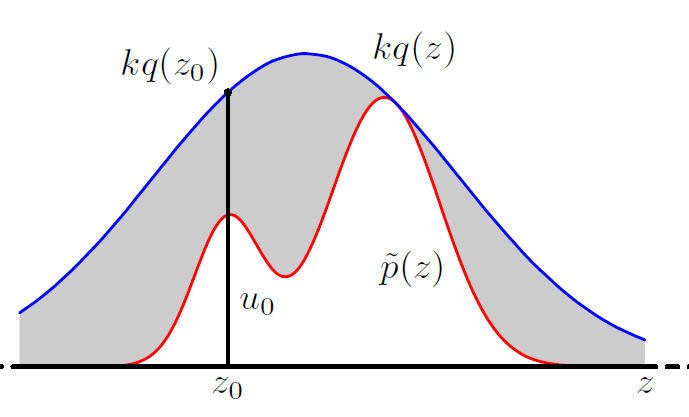
\includegraphics[width=0.9\textwidth]{images/rjsampling2}
\end{center}

\end{frame}



\begin{frame}
    \frametitle{Raytracing}
\framesubtitle{}
\begin{block}{Pathtracing}
Die Anwendung der Monte Carlo Integration auf die Pfadformulierung der Rendergleichung wird Pathtracing genannt.
\end{block}
\end{frame}




\begin{frame}
    \frametitle{Raytracing}
\framesubtitle{}
Wenige und viele samples im Vergleich

    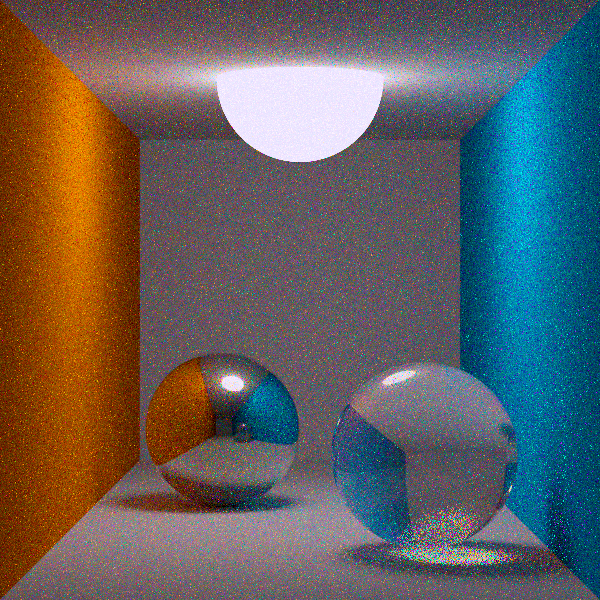
\includegraphics[width=0.45\textwidth]{images/Path_Tracing_Low}
    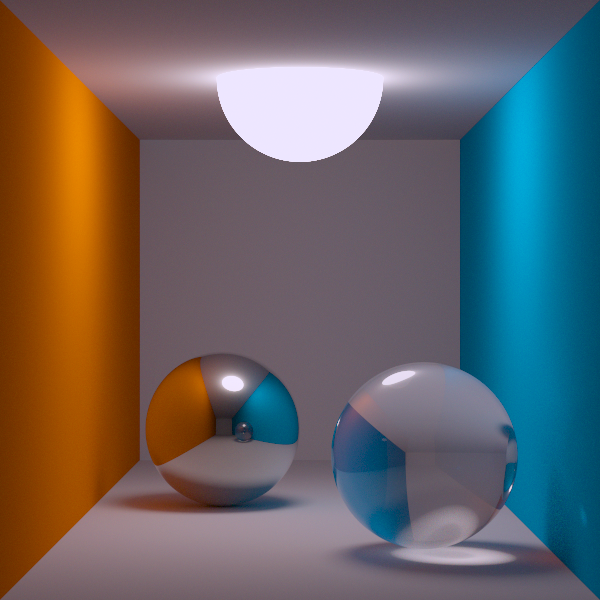
\includegraphics[width=0.45\textwidth]{images/Path_Tracing_High}

\end{frame}



\end{document}
